\subsection{Evolution System}

The formulation employed in this chapter was initially developed and published in Ref.~\cite{PhysRevD.96.104040}. Although the primary focus of that publication differs from the subject matter of this chapter, Appendix A of the paper contains the 3+1 decomposed Klein-Gordon equation for a massive scalar field, as presented in equations A3c and A3d. For the sake of completeness, these equations are
%
\begin{align}
  \partial_t \Phi =   & -2 \alpha K_\phi + \mathcal{L}_\beta \Phi \label{eq:wave_scattering_a3c}                                                                                                                                                     \\
  \partial_t K_\Phi = & \alpha \left( K K_\Phi - \frac{1}{2} \gamma^{ij} D_i \partial_j \Phi + \frac{1}{2} \mu^2 \Phi \right) - \frac{1}{2} \gamma^{ij} \partial_i \alpha \partial_j \Phi + \mathcal{L}_\beta K_\Phi, \label{eq:wave_scattering_a3d}
\end{align}
%
where $\Phi$ is the scalar field being evolved, $K_\Phi$ its ``canonical momentum'', given by
%
\begin{equation}
  K_\Phi = -\frac{1}{2\alpha} \left( \partial_t - \mathcal{L}_\beta \right)\Phi,
  \label{eq:wave_scattering_a2}
\end{equation}
%
$\alpha$ is the spacetime lapse, $\beta^i$ its shift vector, $\gamma^{ij}$ its induced 3-metric, $K$ the trace of its extrinsic curvature tensor, $D_i$ the covariant derivative associated with $\gamma^{ij}$, $\mu$ the spacetime mass parameter and $\mathcal{L}_\beta$ is the Lie derivative along the shift vector $\beta^i$, given explicitly by
%
\begin{equation}
  \mathcal{L}_\beta\Phi = \beta^i \partial_i \Phi.
  \label{eq:wave_scattering_lie_derivative}
\end{equation}

To expand each component of these equations, we utilized the mathematical software package \texttt{Wolfram Mathematica}. The resulting expansion was subsequently implemented into the \texttt{Thorn} by automatically generating corresponding \texttt{C} code from within \texttt{Mathematica}. The code used in this process can be found in \texttt{Notebooks/equations.nb} of the \texttt{Thorn}'s repository.

\subsection{Initial data}

The implementation supports three distinct initial conditions for the scalar field and its canonical momentum. These include a plane wave, an exact Gaussian, and a multipolar Gaussian function. The plane wave and exact Gaussian initial data were developed for the purpose of testing multipatch derivatives in flat spacetime, which will be elaborated on further in subsequent sections. The exact Gaussian initial data is named as such to reflect the fact that it is an exact solution of the Klein-Gordon equation in flat spacetime.

The multipolar Gaussian function is a basic Gaussian function that is multiplied by a linear combination of real spherical harmonics. This particular function was the one chosen during our ``production'' runs as it has the ability to excite specific modes in the system based on the chosen parameters for the linear combination. The development of this initial data is based on the methodology presented in Ref.~\cite{PhysRevD.87.043513}. Explicitly, the multipolar Gaussian function $M_G$ is written as
%
\begin{equation}
  M_G(x, y, z) = \sum_{l=0}^{N}\sum_{m = -l}^{l} c_{l m} Y_{l m}(X,Y,Z) G(R-R_0,\sigma)
  \label{eq:wave_scattering_multipolar_gaussian}
\end{equation}
%
where $X = x - x_0$, $Y = y - y0$, $Z = z - z0$, $R = \sqrt{X^2 + Y^2 + Z ^2}$, $Y_{lm}(x, y, z)$ are the real spherical harmonics, given by
%
\begin{equation}
  Y_{lm}(x, y, z) =
  \begin{cases}
    (-1)^m \sqrt{\frac{2 l + 1}{4\pi} \frac{(l-m)!}{(l+m)!}} P_{lm}\left( \frac{z}{\sqrt{x^2 + y^2 + z^2}} \right) \cos(m \arctan(y,x)) \text{ if } m \geq 0      \\
    (-1)^m \sqrt{\frac{2 l + 1}{4\pi} \frac{(l-|m|)!}{(l+|m|)!}} P_{l|m|}\left( \frac{z}{\sqrt{x^2 + y^2 + z^2}} \right) \sin(|m| \arctan(y,x)) \text{ if } m < 0 \\
  \end{cases}
  ,
  \label{eq:wave_scattering_real_spherical_harmonics}
\end{equation}
%
$G(r, \sigma)$ is the standard Gaussian function, given by
%
\begin{equation}
  G(r, \sigma) = \exp\left( -\frac{1}{2} \left( \frac{r}{\sigma} \right)^2  \right).
  \label{eq:wave_scattering_gaussian}
\end{equation}
%
The parameters $(x_0, y_0, z_0)$ are the center of the multipolar Gaussian, $R_0$ its radius and $\sigma$ the Gaussian width. Once again, code generation routines for the initial data can be found in \texttt{Notebooks/equation.nb}

\begin{figure}[!ht]
  \centering
  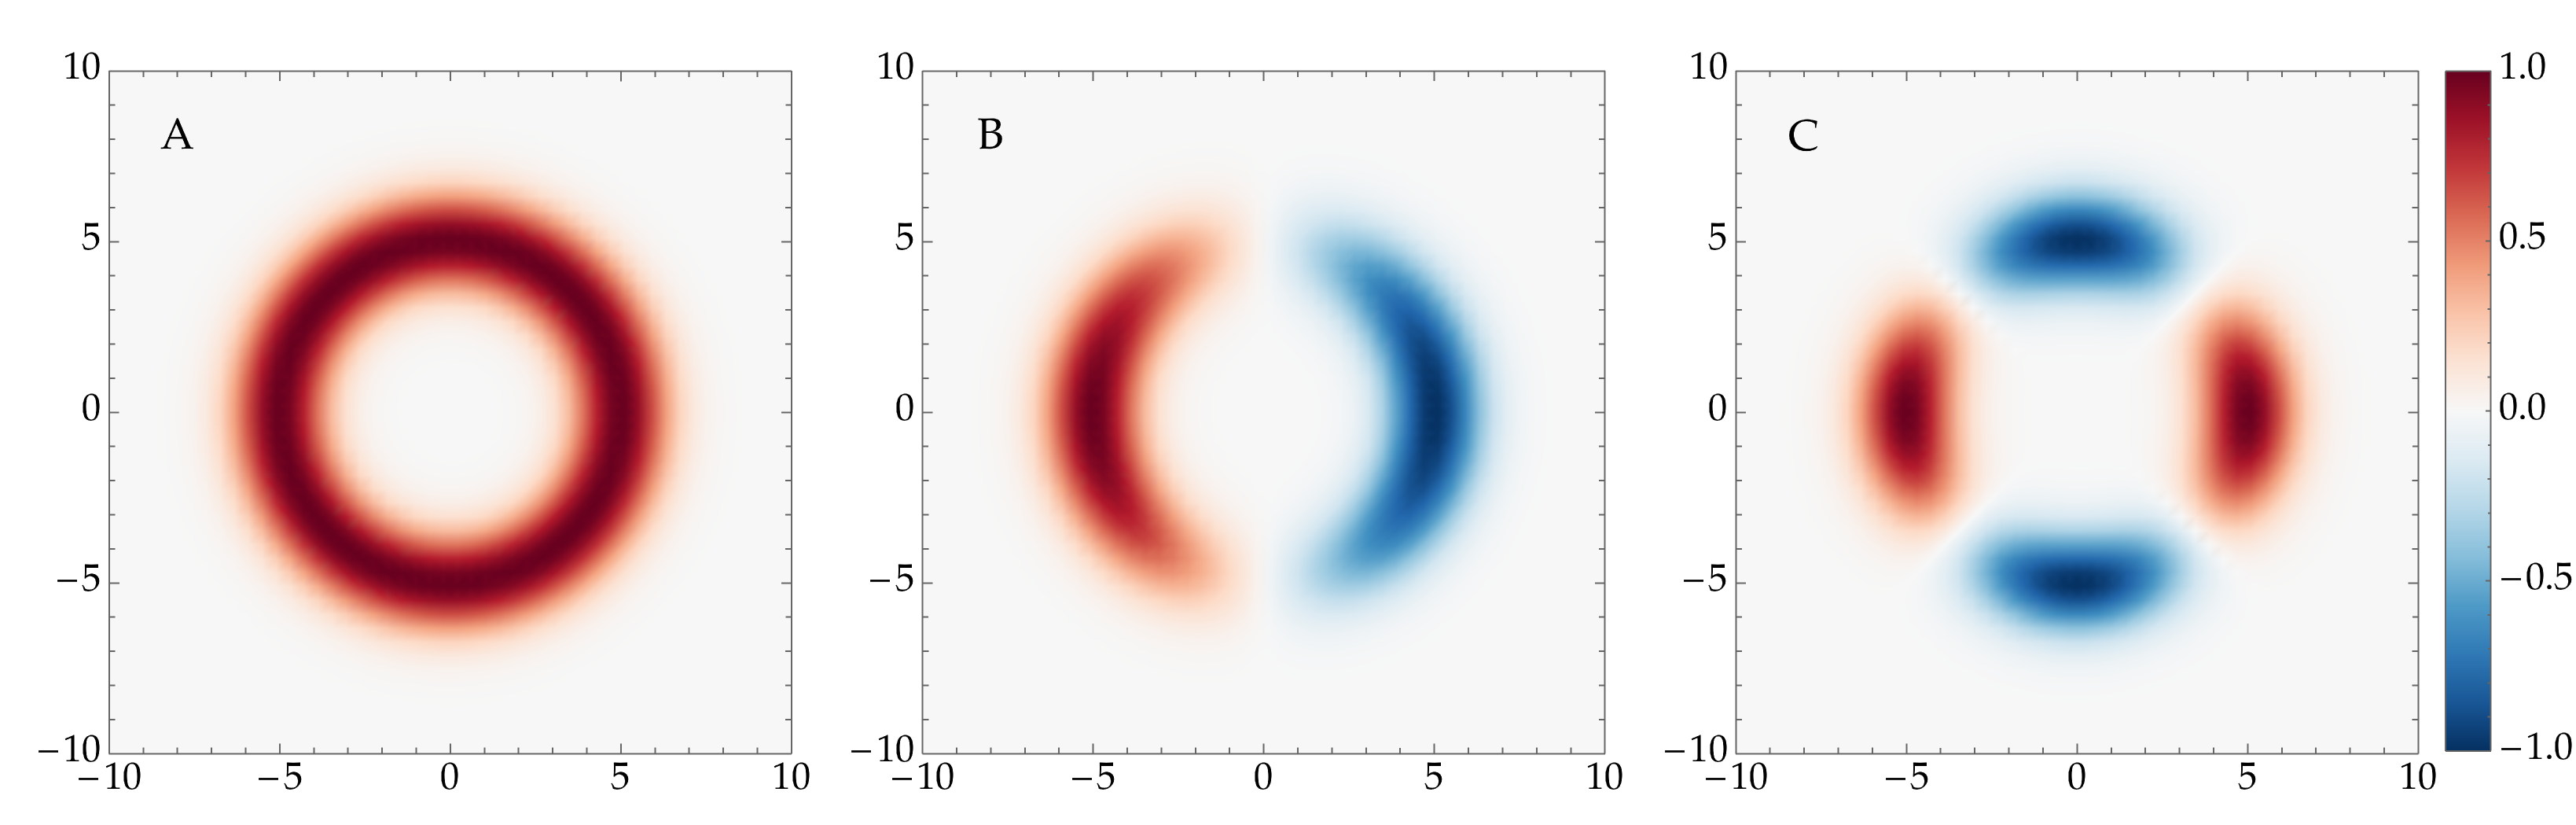
\includegraphics[width=\linewidth]{img/wave_scattering/multipolar_gaussian_id_examples.png}
  \caption{TODO.}
  \label{fig:arrays_steps}
\end{figure}